\newpage

\section{Проектирование системы}

\subsection{Проектирование архитектуры ПО (модули)}

\subsubsection*{Иерархия модулей и подмодулей разрабатываемой программы для frontend}

Информационная система включает в себя следующие модули на frontend:

\begin{itemize}
    \item \textbf{Error404} - модуль не найденной страницы
    \item \textbf{Singin} - модуль авторизации
    \item \textbf{Singout} - модуль выхода
    \item \textbf{Product} - модуль для продукта
    \item \textbf{Product/add} - модуль, реализующий добавление новых записей в базу данных;
    \item \textbf{Product/get} - модуль организации локальной базы данных с выводом информации о товарах;
    \item \textbf{Product/get/delete} - модуль удаления записи из локальной базы данных;
    \item \textbf{Product/edit} - модуль, осуществляющий изменение записи;
    \item \textbf{Product/download\_json} - модуль, осуществляющий сохранение данных в JSON;
    \item \textbf{Product/download\_csv} - модуль, осуществляющий сохранение данных в CSV;
    \item \textbf{Product/open} - модуль, осуществляющий открытие файла JSON.
    \item \textbf{Nav} - модуль меню
\end{itemize}

Схема frontend модулей изображена на
\textbf{рис. \ref{fig:gpi_frontend_modules} (стр. \pageref{fig:gpi_frontend_modules})}.

\begin{figure}[!hp]
    \centering
    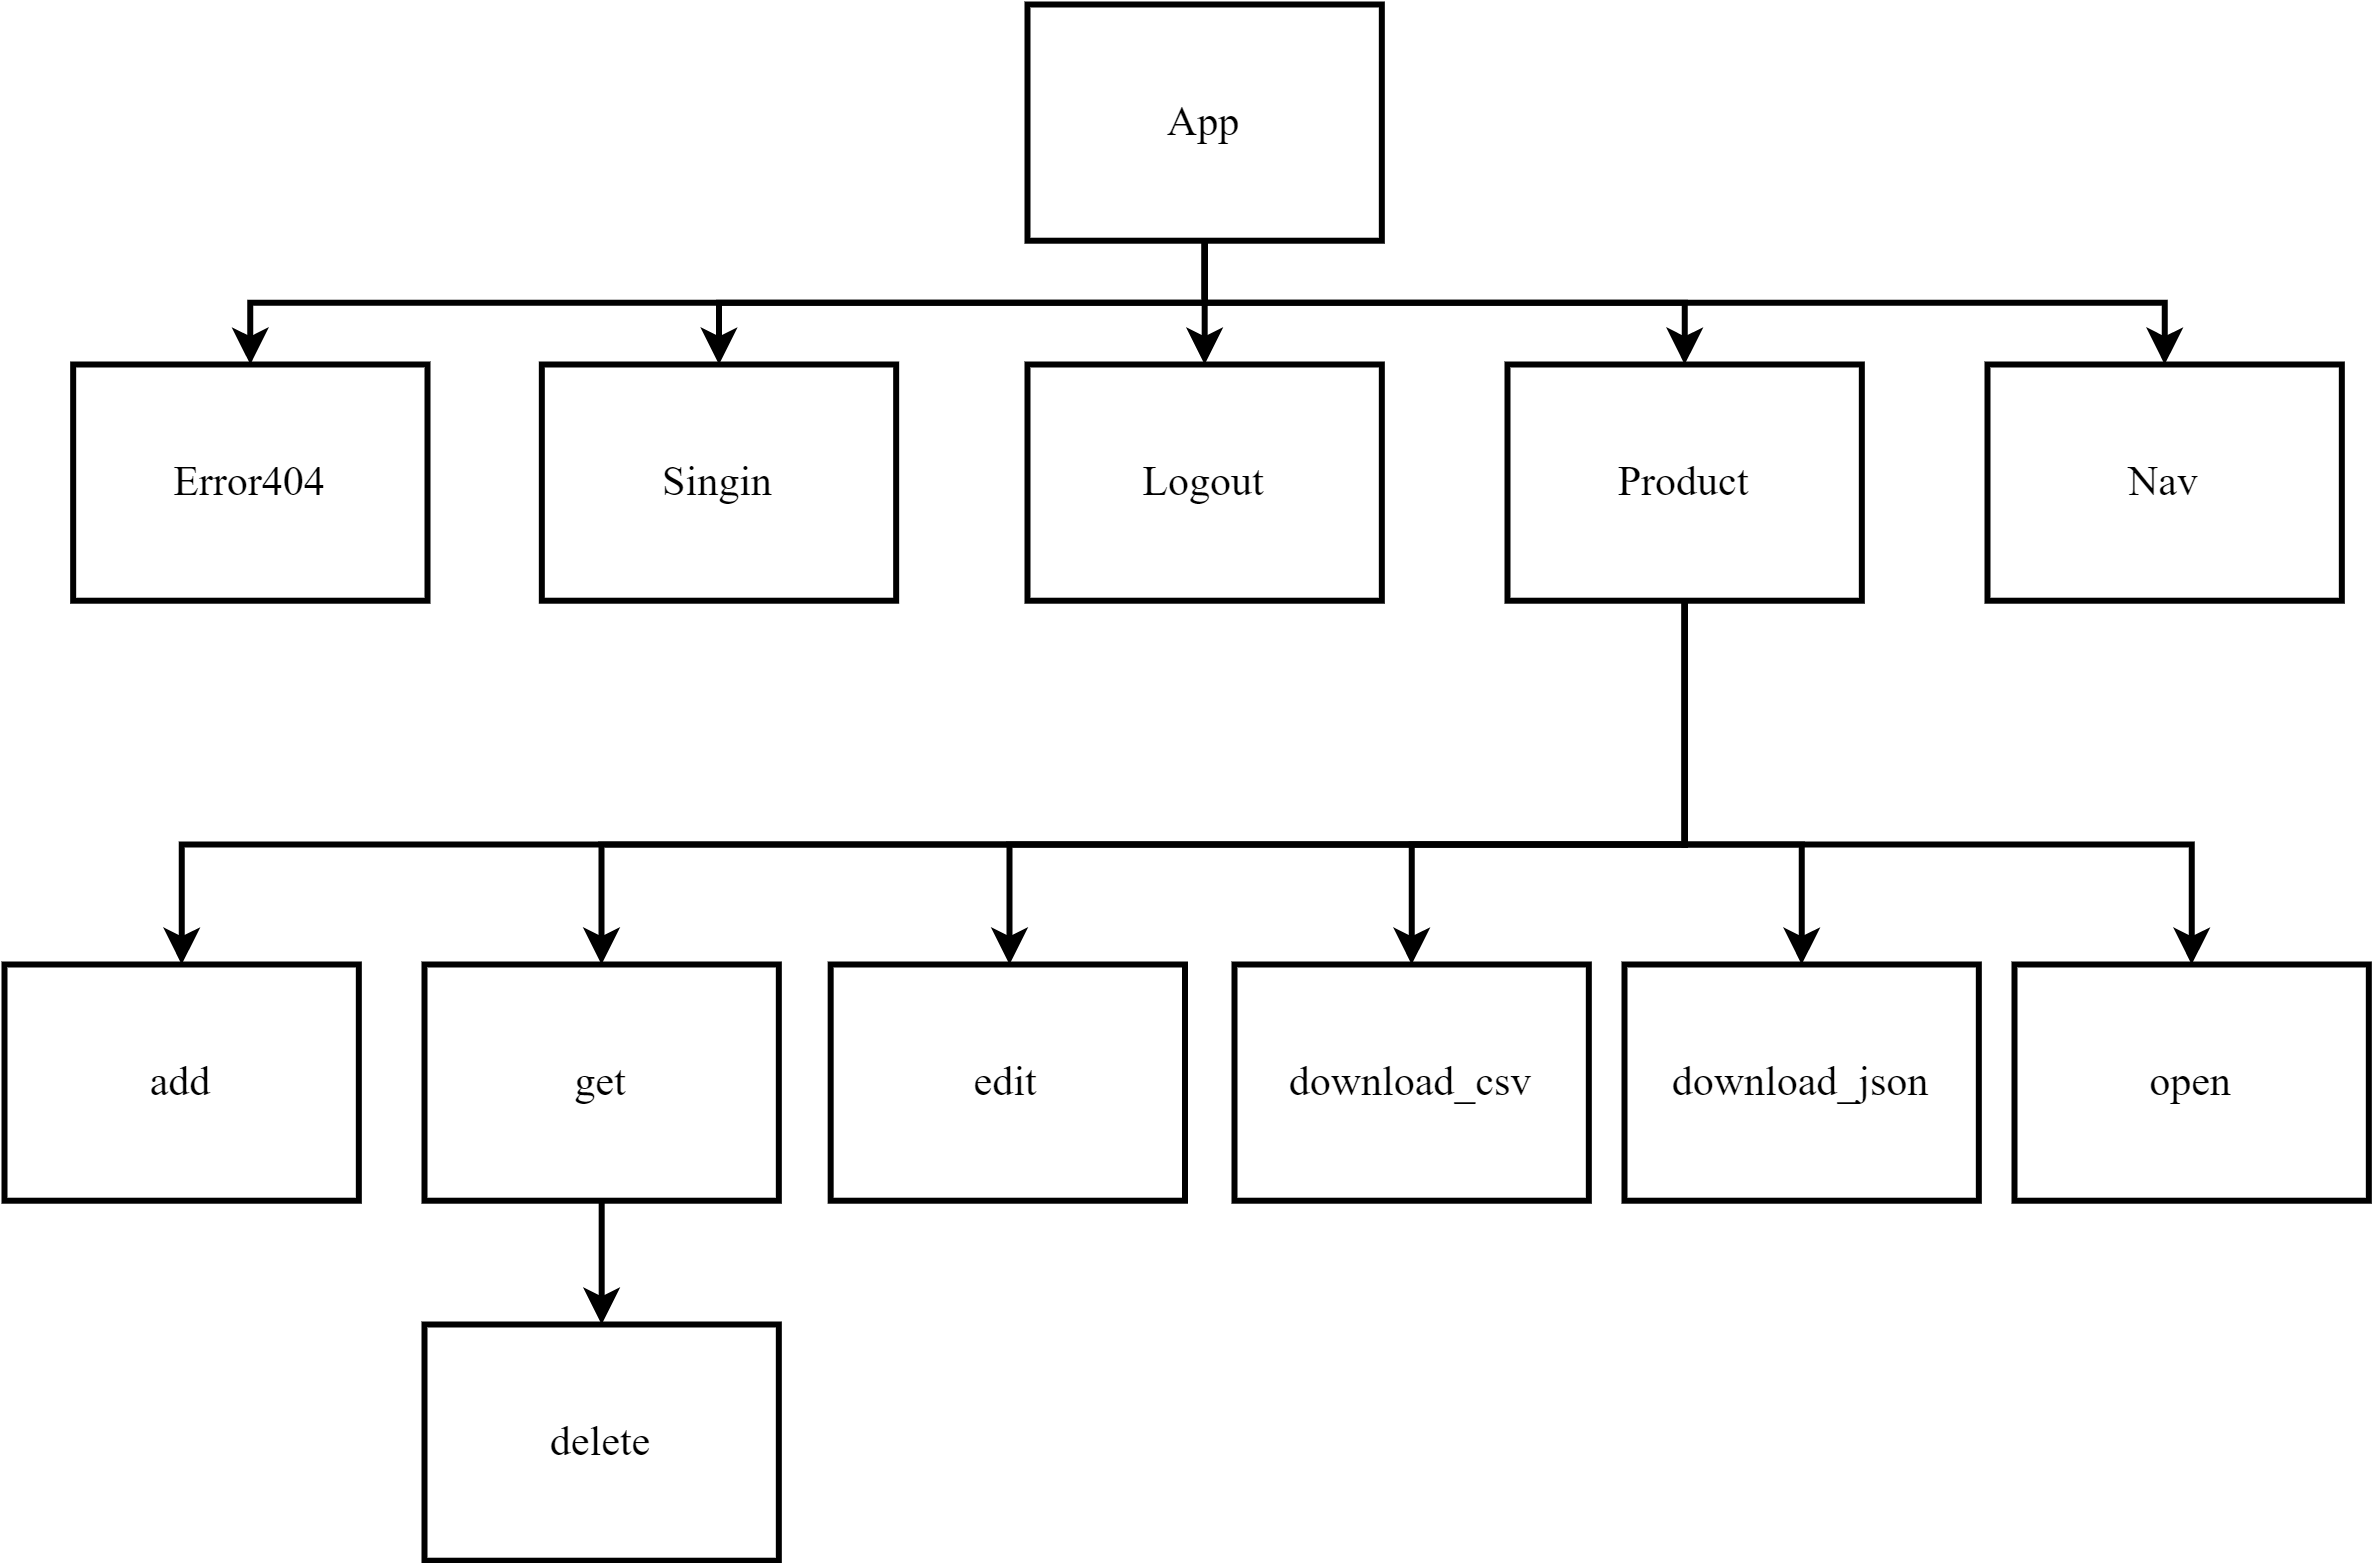
\includegraphics[width=16cm]
        {_assets/gpi_frontend_modules.png}
    \caption{Модули и подмодули для frontend}
    \label{fig:gpi_frontend_modules}
\end{figure}

\subsubsection*{Иерархия модулей и подмодулей разрабатываемой программы для backend}

Информационная система включает в себя следующие модули на backend:

\begin{itemize}
    \item \textbf{products/add} - модуль добавления элементов в базу данных;
    \item \textbf{products/get} - модуль вывода элементов сортированных, инвертированных или по ID;
    \item \textbf{products/edit} - модуль редактирования элемента по ID;
    \item \textbf{products/delete} - модуль удаления элемента по ID.
    \item \textbf{singin} - модуль авторизации;
\end{itemize}

Схема backend модулей изображена на
\textbf{рис. \ref{fig:gpi_backend_modules} (стр. \pageref{fig:gpi_backend_modules})}.

\begin{figure}[!hp]
    \centering
    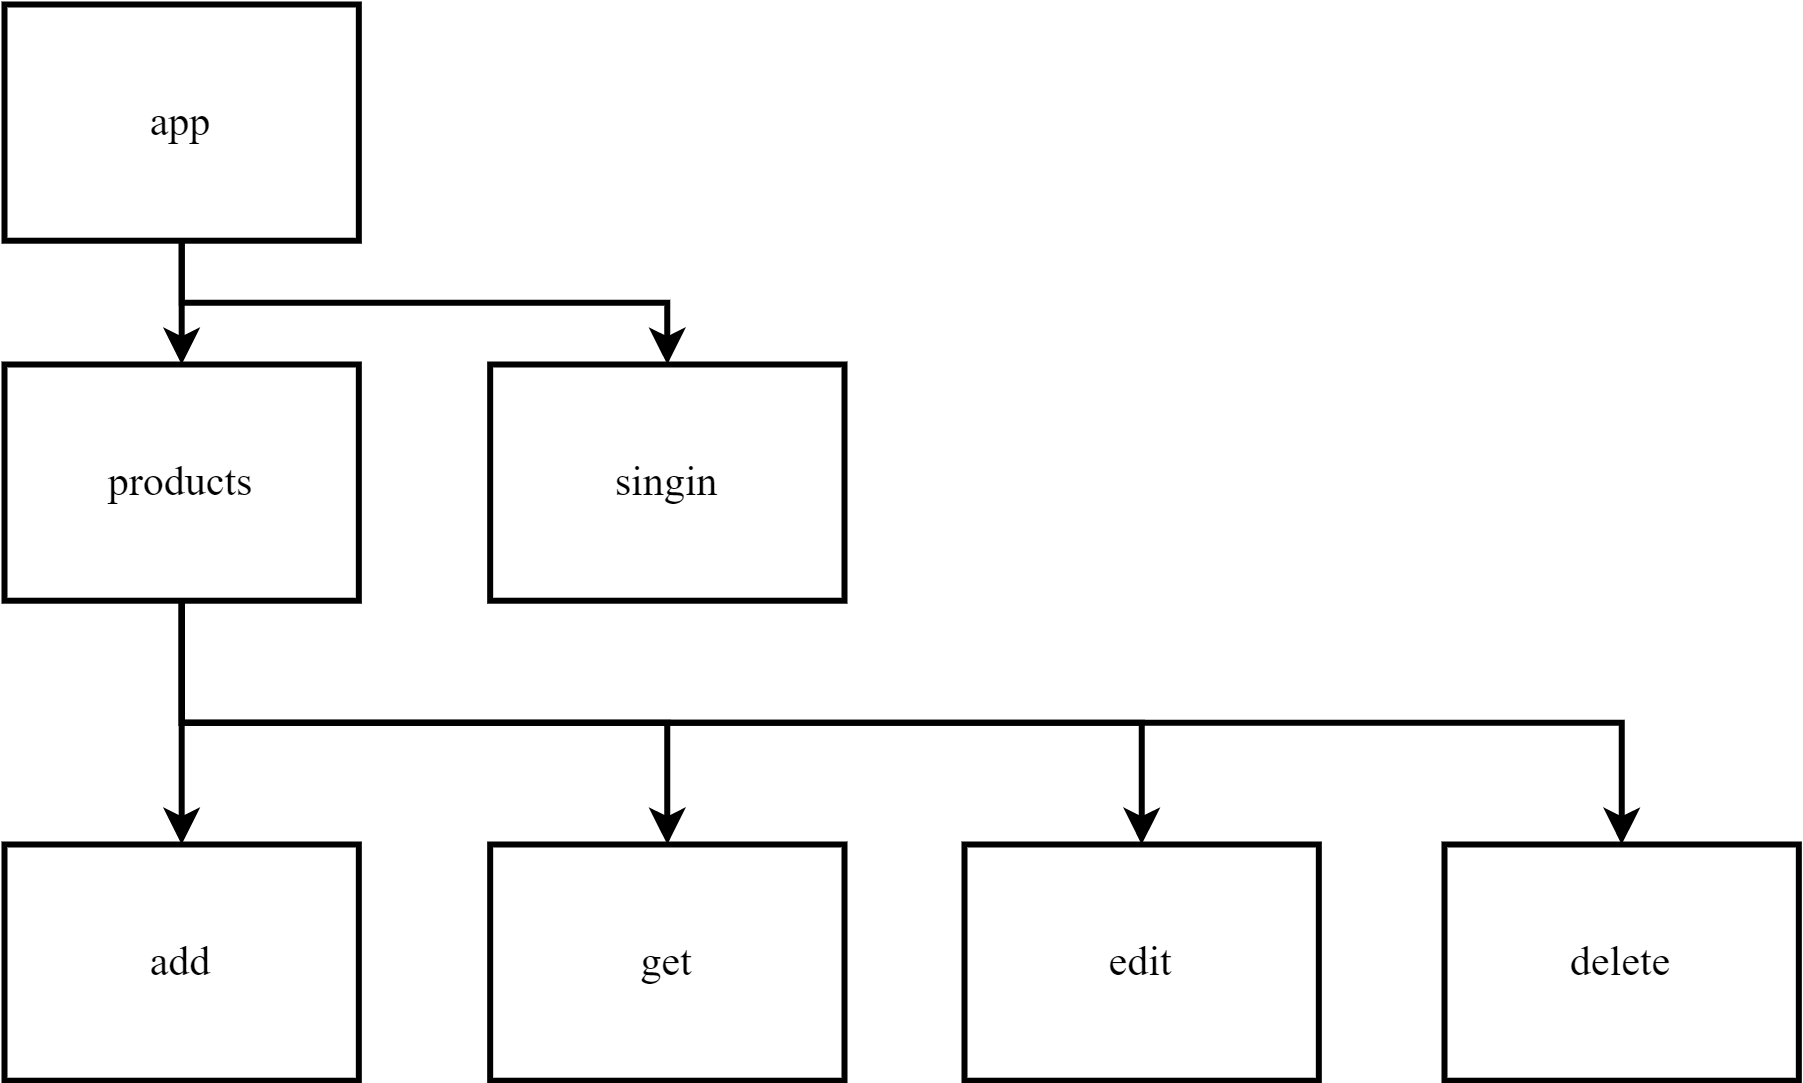
\includegraphics[width=16cm]
        {_assets/gpi_backend_modules.png}
    \caption{Модули и подмодули для backend}
    \label{fig:gpi_backend_modules}
\end{figure}

\newpage

\subsection{Проект. Схема данных}

Трёхуровневая архитектура - архитектурная модель программного комплекса,
предполагающая наличие в нём трёх компонентов: клиента, сервера приложений
(к которому подключено клиентское приложение) и сервера баз данных.

Если мы посмотрим на данную архитектуру с позиции сайта.
То первый уровень можно считать браузером (frontend), с помощью которого посетитель заходит на сайт,
второй уровень - это Express server (backend), а третий уровень - это база данных MySQL.

Схема архитуктуры ПО изображена на
\textbf{рис. \ref{fig:gpi_client_server} (стр. \pageref{fig:gpi_client_server})}.

\begin{figure}[!hp]
    \centering
    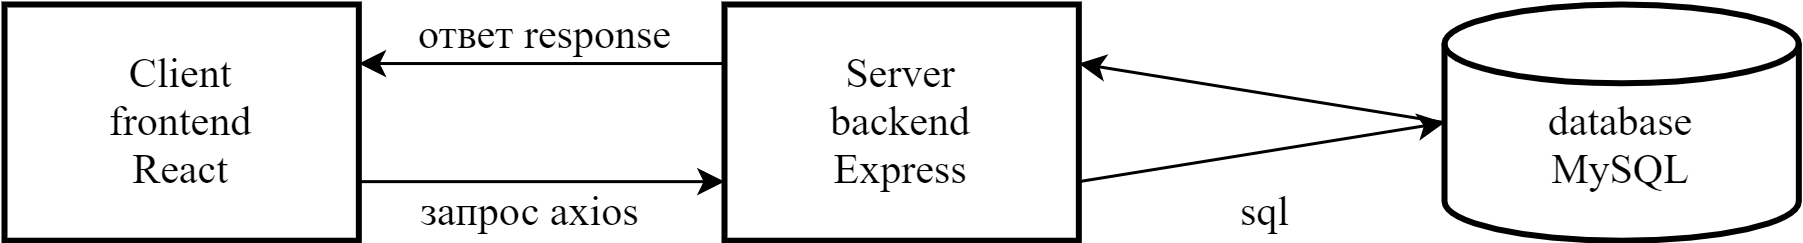
\includegraphics[width=16cm]
        {_assets/gpi_client_server.png}
    \caption{Схема архитектуры ПО}
    \label{fig:gpi_client_server}
\end{figure}

Объект контактов изображен на
\textbf{рис.~\ref{fig:gpi_a_contacts}~(стр.~\pageref{fig:gpi_a_contacts})}

\begin{figure}[!hp]
    \centering
    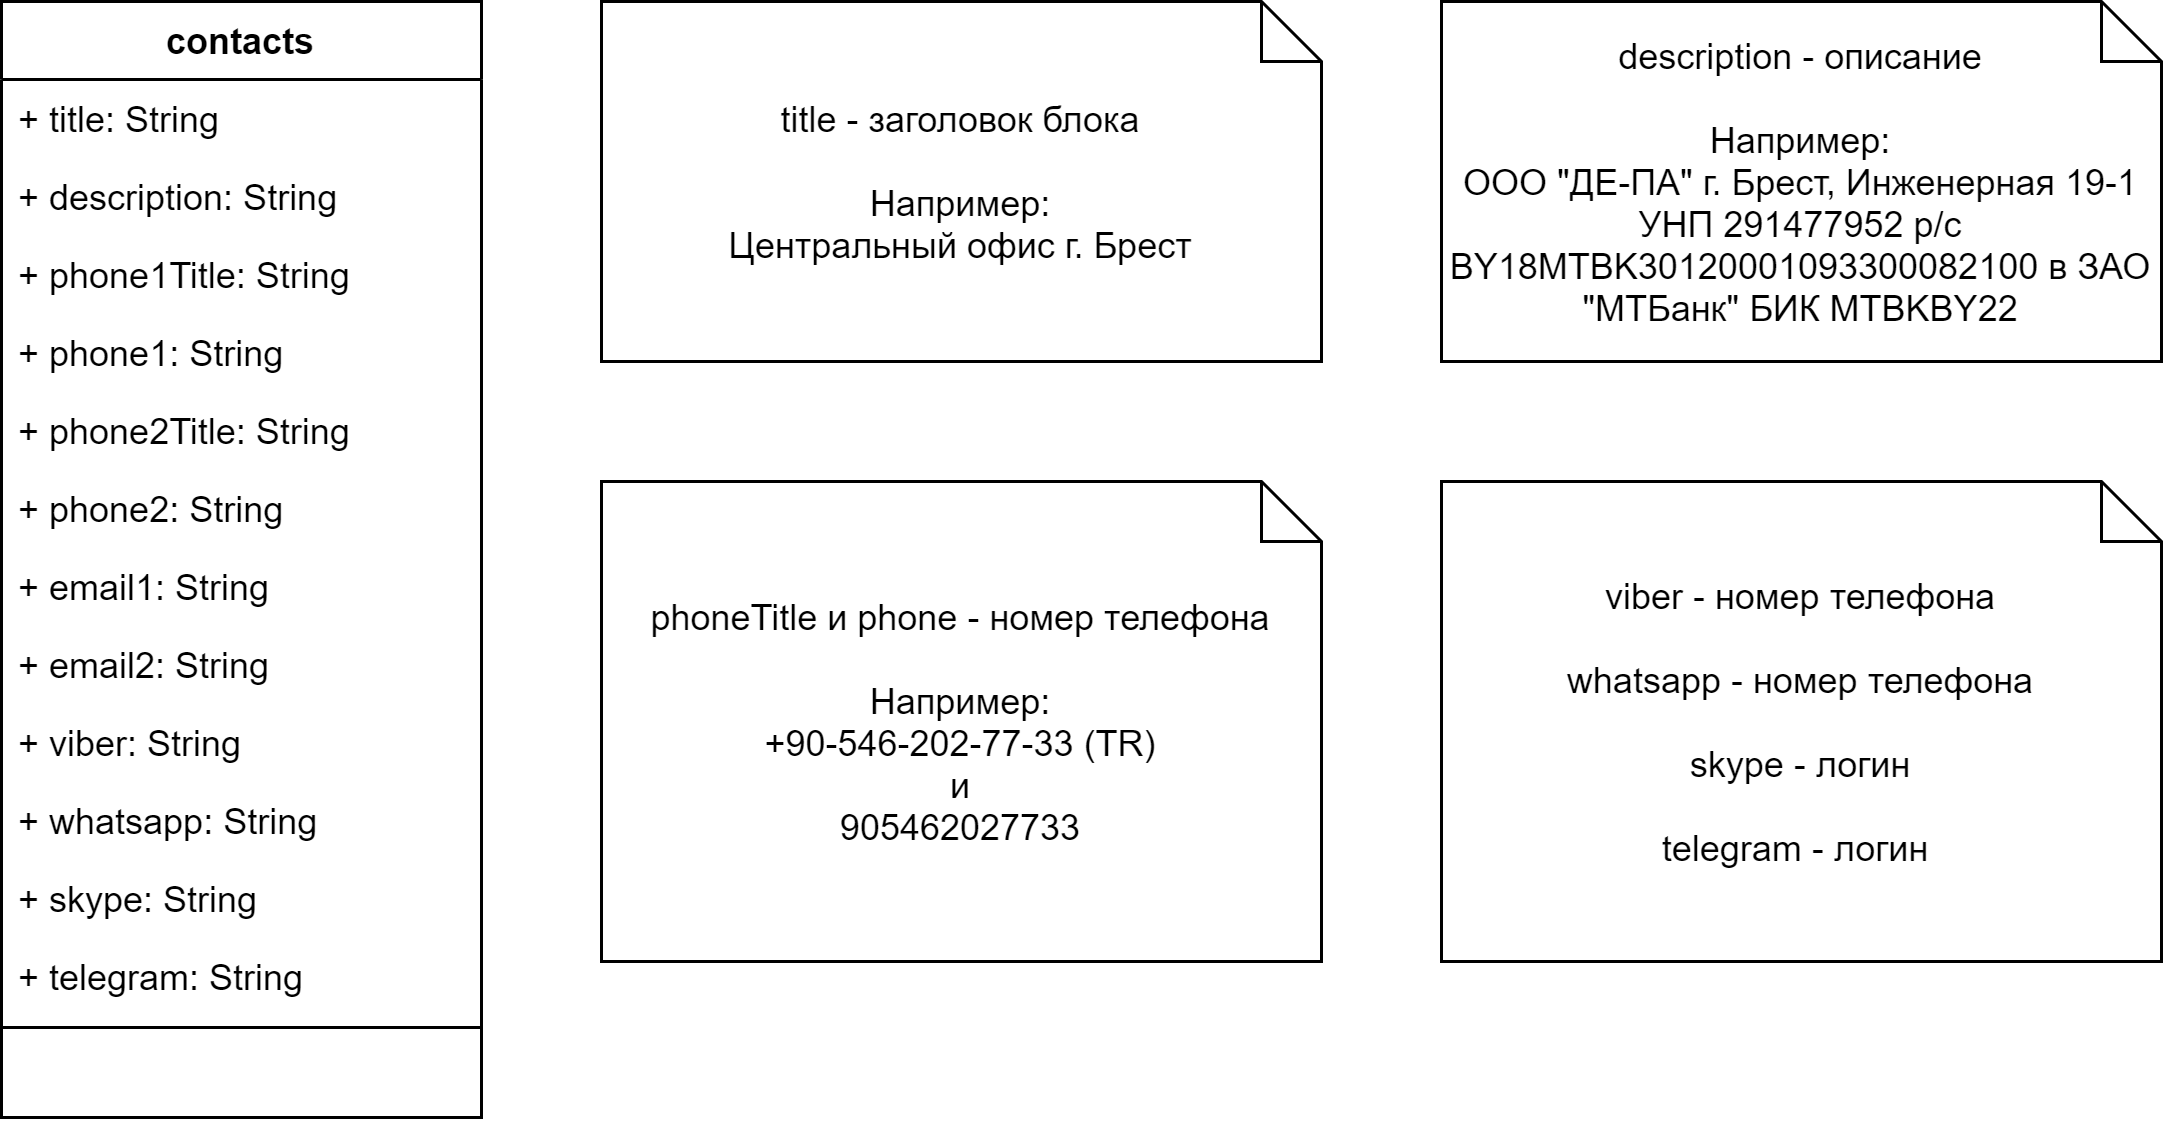
\includegraphics[width=16cm]
        {_assets/gpi_a_contacts.png}
    \caption{Объект контакты}
    \label{fig:gpi_a_contacts}
\end{figure}

Объект документа PDF изображен на
\textbf{рис.~\ref{fig:gpi_a_pdf}~(стр.~\pageref{fig:gpi_a_pdf})}

\begin{figure}[!hp]
    \centering
    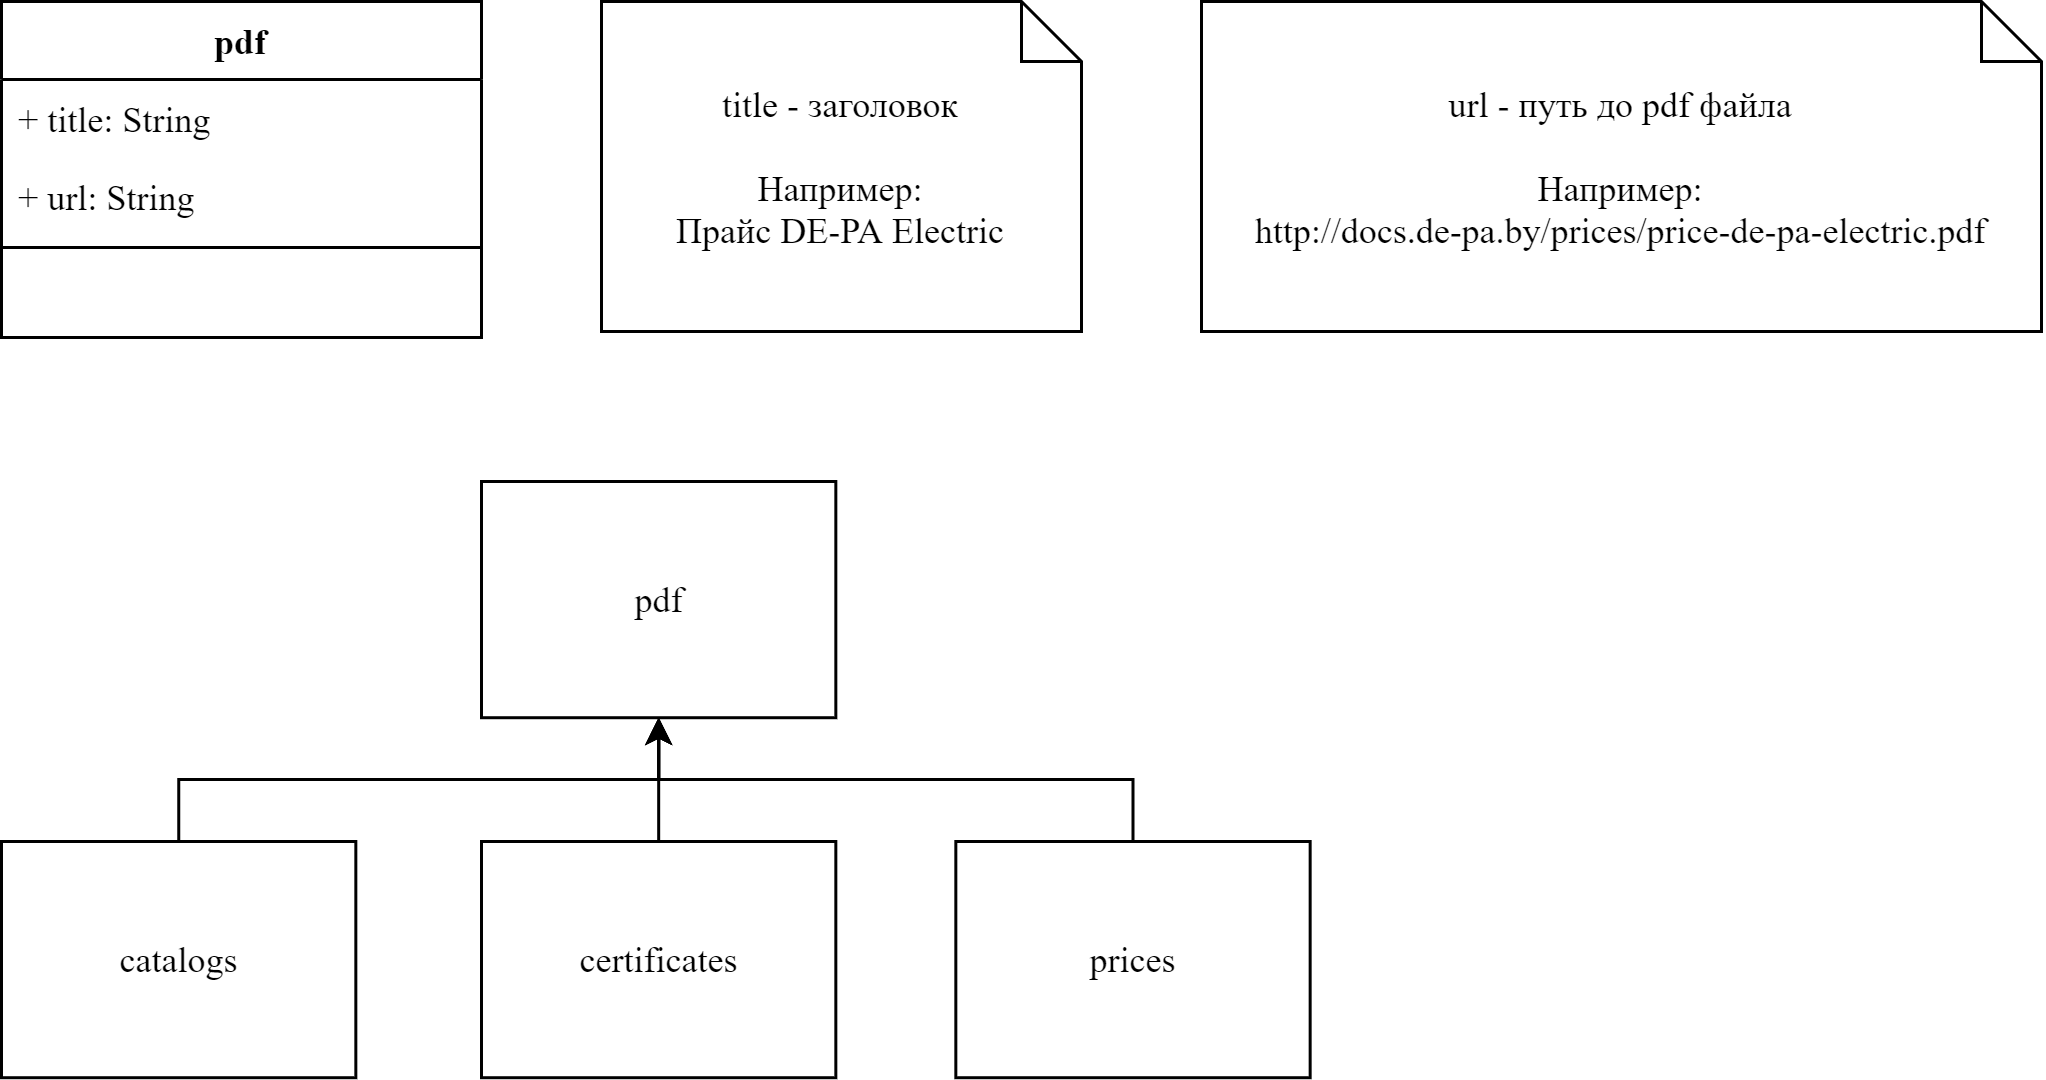
\includegraphics[width=16cm]
        {_assets/gpi_a_pdf.png}
    \caption{Объект документа PDF}
    \label{fig:gpi_a_pdf}
\end{figure}

Объект продукта изображен на
\textbf{рис.~\ref{fig:gpi_a_product}~(стр.~\pageref{fig:gpi_a_product})}

\begin{figure}[!hp]
    \centering
    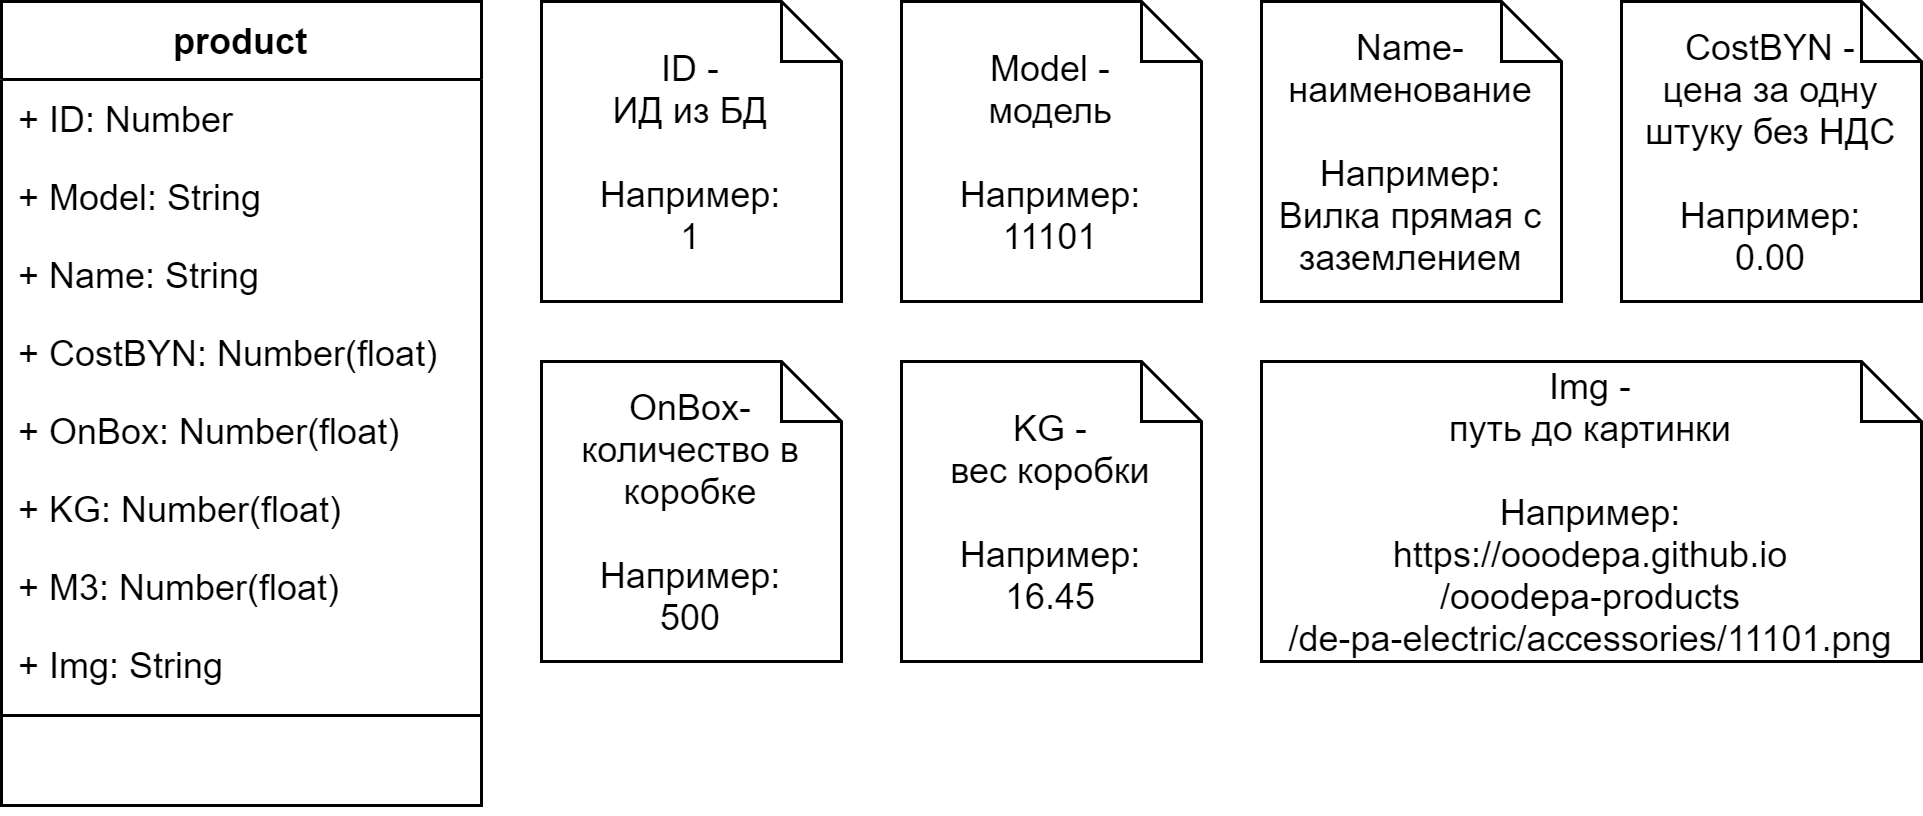
\includegraphics[width=16cm]
        {_assets/gpi_a_product.png}
    \caption{Объект продукта}
    \label{fig:gpi_a_product}
\end{figure}

\newpage

\subsection{Проектирование UI (макеты)}

Макет меню для компьютера изображен на
\textbf{рис.~\ref{fig:gpi_ui_menu}~(стр.~\pageref{fig:gpi_ui_menu})}.

\begin{figure}[!hp]
    \centering
    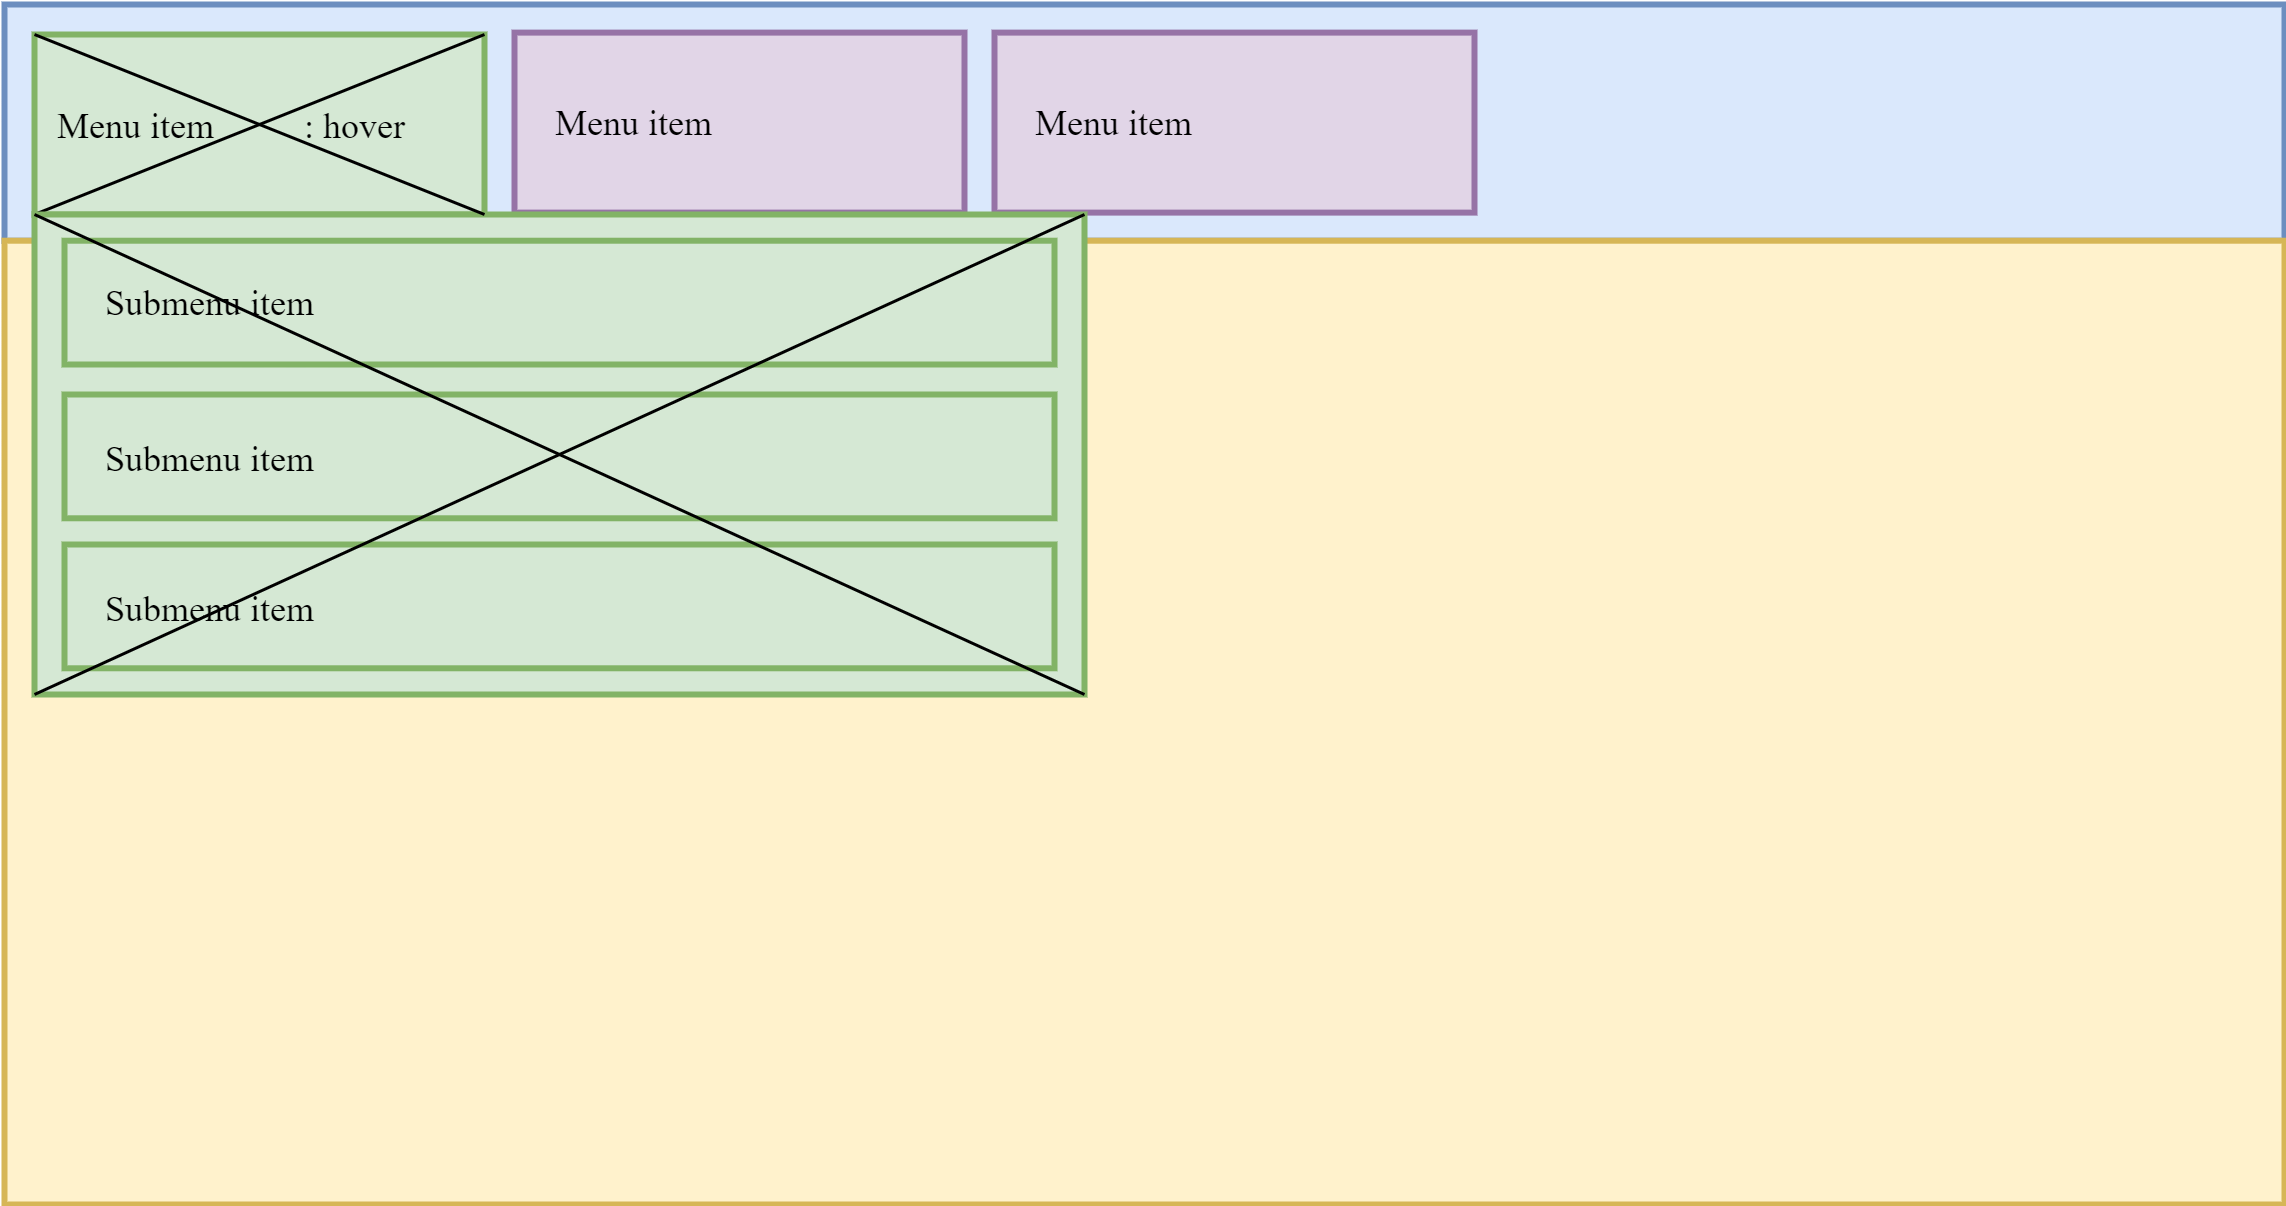
\includegraphics[width=12cm]
        {_assets/gpi_ui_menu.png}
    \caption{Макет мeню для компьютера}
    \label{fig:gpi_ui_menu}
\end{figure}

Макет страницы с таблицей для компьютера изображен на
\textbf{рис.~\ref{fig:gpi_ui_get}~(стр.~\pageref{fig:gpi_ui_get})}.

\begin{figure}[!hp]
    \centering
    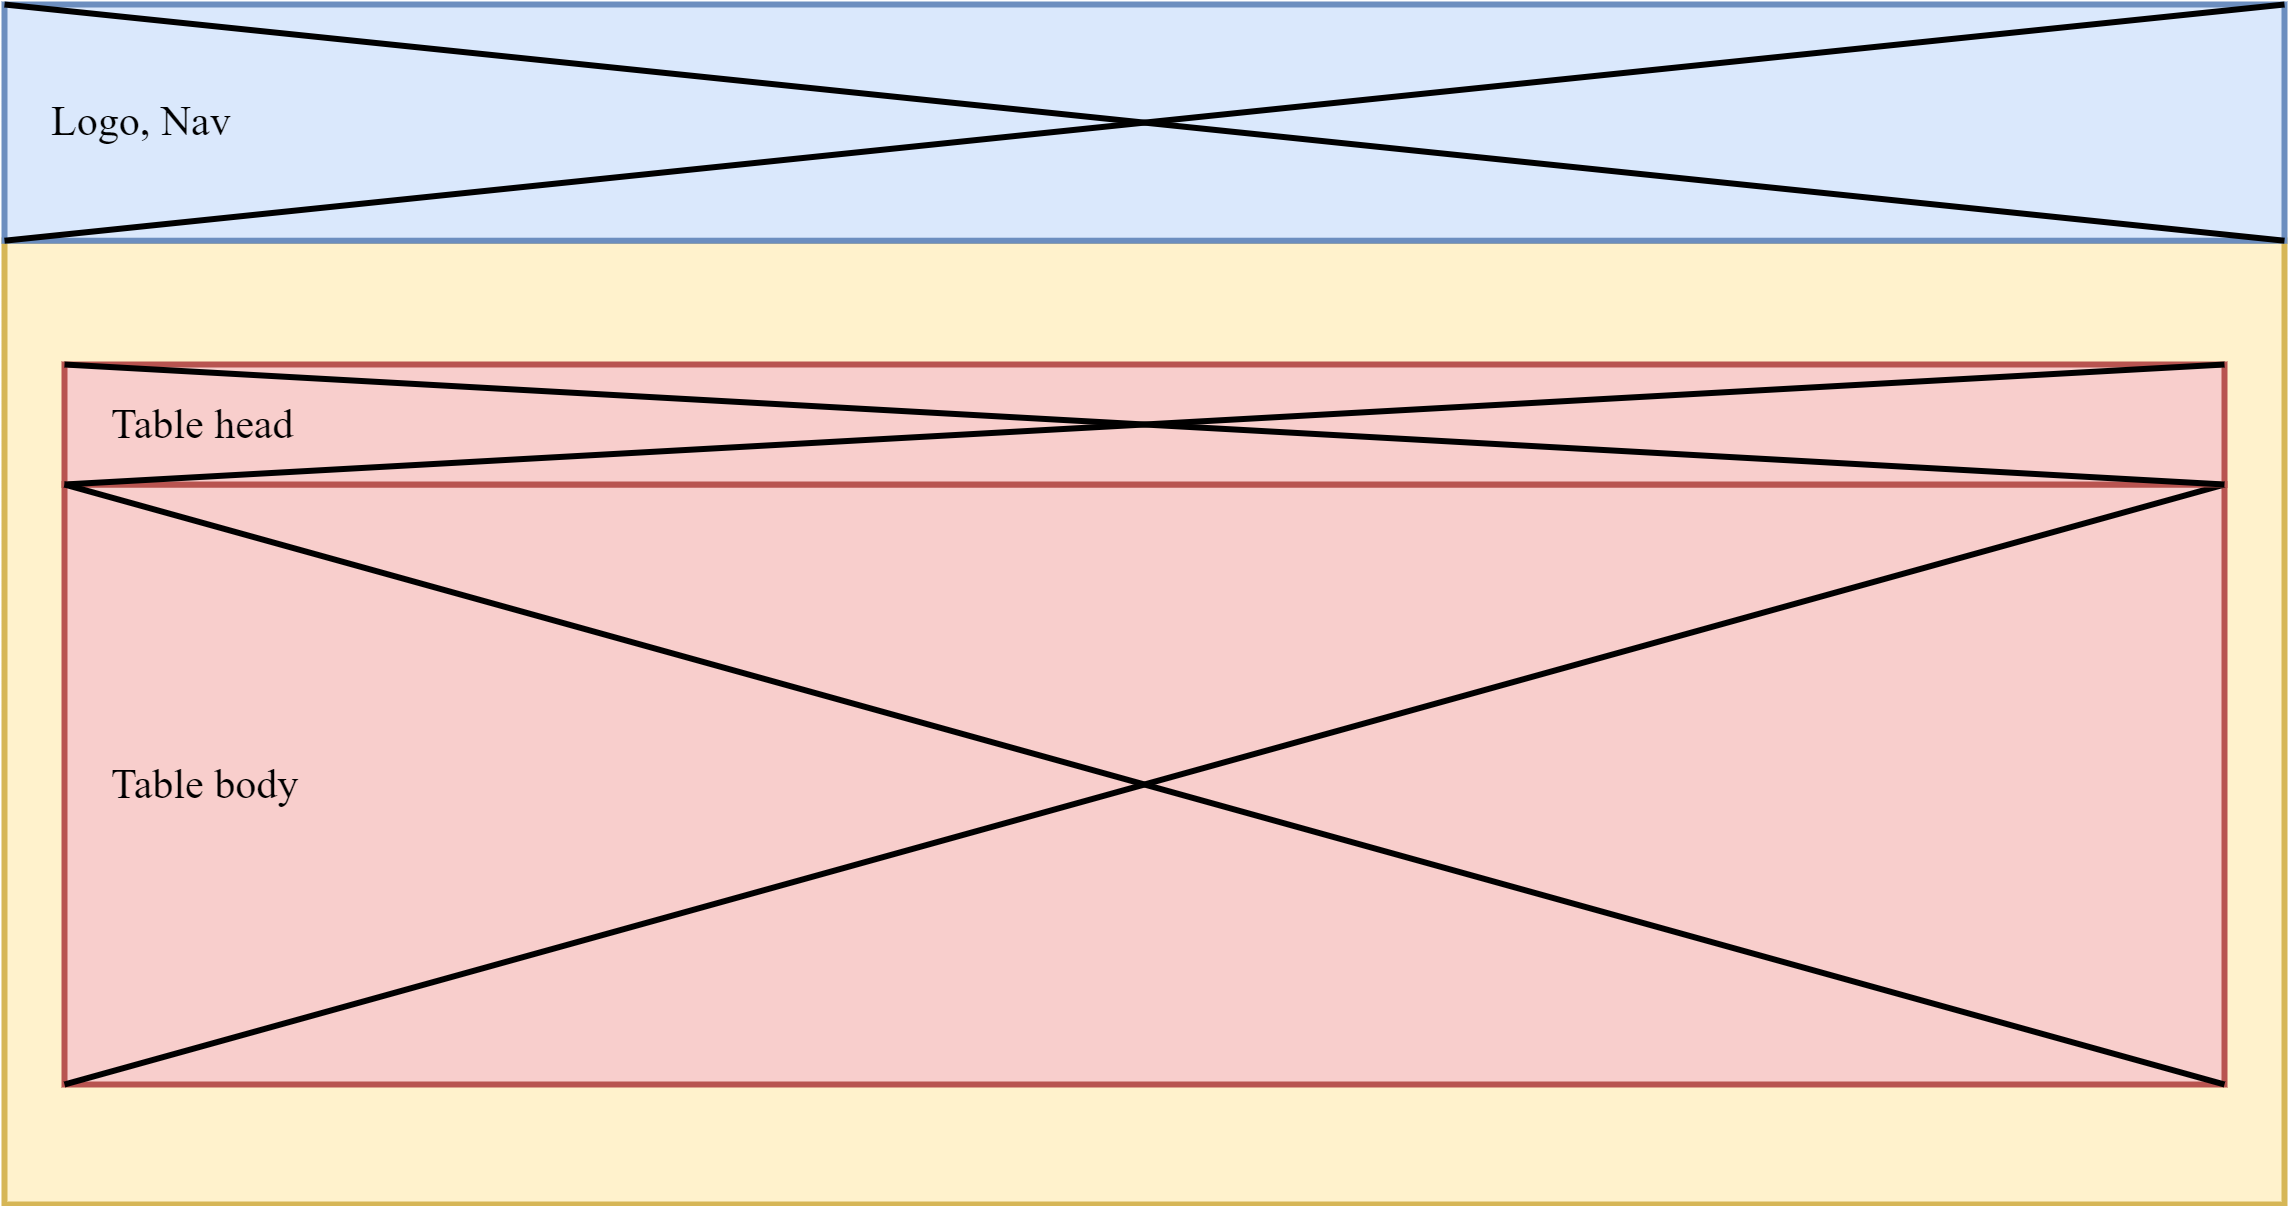
\includegraphics[width=12cm]
        {_assets/gpi_ui_get.png}
    \caption{Макет страницы с таблицей для компьютера}
    \label{fig:gpi_ui_get}
\end{figure}

Макет меню для телефона изображен на
\textbf{рис. \ref{fig:gpi_pz_phone_menu} (стр. \pageref{fig:gpi_pz_phone_menu})}.

\begin{figure}[!hp]
    \centering
    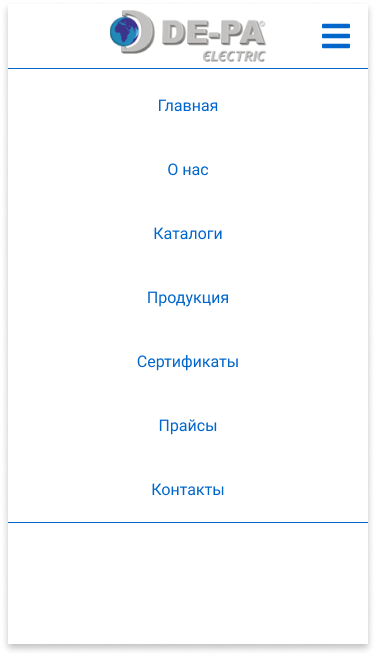
\includegraphics[height=16cm]
        {_assets/gpi_pz_android_menu.png}
    \caption{Макет меню для телефона}
    \label{fig:gpi_pz_phone_menu}
\end{figure}

\newpage
